\chapter{Methodik}
\label{ch:methodik}
Um eine zustandsbasierte -- und darauf aufbauend eine prädiktive -- Instandhaltung umsetzten zu können, ist es nötig Daten zu gewinnen, die diesen Zustand beschreiben, und ein Model zu erstellen, das diese auswertet. Es folgt eine Beschreibung der Methodik nach der die Ergebnisse aus \cref{ch:modelbewertung} erarbeitet werden. Die Methodik beschränkt sich auf die Entwicklung eines zustandbestimmenden Models.
%===============================================================================
\section{Versuchsaufbau}
\label{sec:versuchsaufbau}
Der in \cref{sec:messdaten} beschriebene Datensatz wird mit folgendem Messaufbau erfasst:

An die Türschließanlage ist eine Druckluftzufuhr angeschlossen, welche die Energie zum Antrieb des Kolbens liefert. Ein Druckregeler regelt den Luftdruck auf ca. \SI{550000}{\pascal} (\SI{80}{psi}). Der Luftstrom wird durch ein 5/2-Wegeventil (Model: VUVS-LK25-B52-D-G14-1B2-S; Fa. Festo) gesteuert, dass magnetisch betätigt wird. Die Ventilstellung bestimmt die Bewegungsrichtung des Kolbens. Zwischen Druckregeler und Wegeventil ist außerdem ein Absperrventil (MFH-3-1/8; Fa. Festo) verbaut. Dieses wird ebenfalls durch einen Elektromagneten betätigt und kappt die Luftzufuhr, wenn das System zum Stillstand gebracht werden soll.

Sämtliche Ventile werden über Relais mit den jeweils nötigen elektrischen Spannungen (\SI{24}{\volt}) versorgt. Die Schaltung der Relais -- und damit die Steuerung der Türschließanlage -- erfolgt durch einen Mikrocontroller vom Typ Arduino Uno (Fa. Az-Delivery). Dieser führt den Programmcode (Datei \enquote{csvwriter.ino}; s. Anhang) zur Versuchsdurchführung aus.  Dazu gehört auch das Auslesen des installierten Beschleunigungssensor und Gyroskops (s.~\cref{fig:beschleunigungssensor}). 

\begin{figure}[ht]
	\centering
	
\includegraphics{FH_Kiel_Logo_deut_rgb.jpg}
	\caption{An Türschließanlage befestigter Beschleunigungssensor}
	\label{fig:beschleunigungssensor}
\end{figure}

Die Position des Beschleunigungssensors ist so gewählt, dass keine konstruktive Änderung an der Türschließanlage vorgenommen werden muss. Abhängig von der Position des Sensors relativ zur Umlenkrolle sind unterschiedliche Messwerte zu erwarten. Da die absoluten Messwerte für die Klassifikation nicht von Bedeutung sind; sondern nur deren Unterschied in Bezug auf die Kategorien; erweist sich die Position des Sensors als geeignet.

Zur Speicherung der Daten werden diese über eine serielle USB-Schnittstelle an ein angeschlossenes Computersystem übertragen. Der dort, parallel laufende Programmcode (Datei: \enquote{csvwriter.py};s. Anhang) decodiert das Signal des Mikrocontrollers und speichert die Daten in einer passend formatierten CSV-Datei ab.

Um vergleichbare Datenpunkte zu erhalten wird für die Messreihe nicht das Original der Umlenkrolle verwendet, sondern mit im Lasersinterverfahren hergestellten Nachbildungen (s.~\cref{fig:seilrolle_isometrisch}). Die Festigkeit des Materials ist für den Versuch ausreichend. Nach dem Versuch wurden bei einer Sichtprüfung keine plastischen Verformungen festgestellt. Eine der Nachbildungen wurde mit Rillen versehen, die längst der Bohrung verlaufen (s.~\cref{fig:seilrolle_rillen}). Die Rillen simulieren Materialausbrüche als Folge von Pittings. Insgesamt weist die so künstlich beschädigte Umlenkrolle drei Rillen auf die um jeweils 45° zueinander verschoben sind.

\begin{figure}[ht]
	\centering
	\subfloat[Unbeschädigte Nachbildung der Seilrolle\label{fig:seilrolle_isometrisch}]{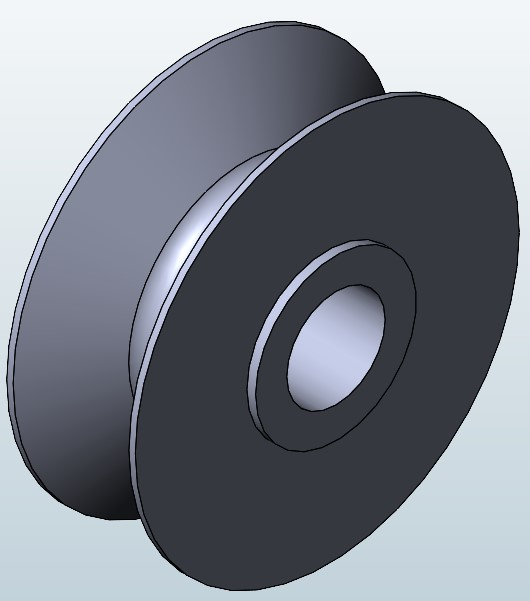
\includegraphics[width=0.35\textwidth]{seilrolle_isometrisch.jpg}}
	\qquad
	\subfloat[Rillen in künstlich beschädigten Nachbildung\label{fig:seilrolle_rillen}]{\includegraphics[width=0.43\textwidth]{seilrolle_rillen_bemaßt.jpg}}
	\caption{Nachbildungen der Umlenkrolle}
	\label{fig:cad_seilrolle}
\end{figure}

Mit verbauter intakter bzw. beschädigter Umlenkrolle werden jeweils 100 Datenpunkte aufgezeichnet. Ein Datenpunkt entspricht einem Öffnungs- und Schließvorgang, wie er durch den Programmcode vorgegeben wird.
%===============================================================================
\section{Messwerte und Datenaufbereitung}
\label{sec:messdaten}
Der Datensatz weißt \num{1441} Merkmale auf. Je \num{240} davon bilden eine Zeitreihe einer der Messwerte von Beschleunigungssensor bzw. dem Gyroskop. Insgesamt beinhaltet der Datensatz folgende Messwerte (Achsenrichtungen beziehen sich auf den Beschleunigungssensor):
\begin{itemize}
	\item Beschleunigung aller drei Raumachsen
	\item Rotationgeschwindigkeiten um alle drei Raumachsen
	\item Zykluszeit: Dauer eines Öffnungs- und Schließvorgangs (inkl. Laufzeitpause das Programmcodes)
\end{itemize}

Die Messgrößen der Beschleunigungen und der Rotationgeschwindigkeiten wurden ausgewählt, da sie das Schwingungsprofil der Anlage beschreiben. Es wird erwartet, dass sich dieses mit dem Grad der Beschädigung der Umlenkrollen ändert. Es kann also erwartet werden, dass die gewählten Messgrößen aussagekräftig über den Zustand der Umlenkrollen sind. Voraussetzung ist das, dass eine andere Ursache für die Änderung des Vibrationsprofils nicht in Frage kommt. Diese Voraussetzung ist hier geben, weil die Umlenkrolle die einzige Variable im Versuchsaufbau ist.

Für die Modelentwicklung ist es sinnvoll die Rohdaten in einem beschreibenden Datensatz zusammen zu fassen. Die erstellten Modelle basieren auf Entscheidungsbäumen mit maximal sechs Ebenen (vgl. \cref{sec:modelauswahl} bzw. \cref{sec:modellierung}). Das bedeutet, dass jeder Entscheidungsbaum nur einen sehr kleinen Anteil der Merkmale des Rohdatensatzes verwenden kann. Dies kann eine ungewünschte negative Auswirkung auf die Entwicklung des Models haben. Es besteht die Möglichkeit, dass ein Model nur Merkmale berücksichtigt, die zu dem selben Messwert gehören, weil diese zufällig eine höhe Aussagekraft für die Zuordnung der richtigen Kategorien haben, aber nicht zwangsläufig für die Population gültig sind. Informationsgehalt der anderen Messwerte geht so verloren. Mit einem Datensatz, der die Informationen der Zeitreihen in statistischen Parametern zusammenfasst, kann eine größerer Anteil dieser Merkmale verwendet werden und so mehr Informationen des Rohdatensatzes genutzt werden. Die Entscheidungsbäume der erstellten Modelle besitzen maximal \num{32} Knoten (s.~\cref{sec:modellierung}). Sie können alle Merkmale des beschreibenden Datensatzes nutzen, der insgesamt über \num{25} Merkmale verfügt.

Aus dem genannten Grund wird ein beschreibender Datensatz aus den Rohdaten abgeleitet. Der Datensatz beschreibt die Messungen anhand folgender Parameter (ersten vier je Messgröße).
\begin{itemize}
	\item Minimalwert
	\item Maximalwert
	\item Median
	\item Standardabweichung
	\item Zykluszeit
\end{itemize}
%===============================================================================
\section{Modelauswahl}
\label{sec:modelauswahl}
Die Menge an Klassifikationsmodelle ist größer als sie im Rahmen dieser Arbeit berücksichtigt werden kann. Jedoch kann eine sinnvolle Vorauswahl an geeigneten Modeltypen getroffen werden. So kann die Anzahl der Modelle, die tatsächlich entwickelt und verglichen werden müssen, auf ein handhabbares Maß reduziert werden.

Die Vorauswahl geeigneter Modeltypen richtet sich nach folgenden Anforderungen. Die Anforderungen sind von den Erfolgskriterien Komplexität und Modelqualität des Usecases abgeleitet (vgl.~\cref{sec:erfolgskriterien_usecase}).

\begin{itemize}
    \item Für den vorhandenen Datensatz muss eine hohe Modelqualität erwartet werden können. Die Modelqualität wird für den Usecase durch die Sensitivität und Relevanz der Klassifikation bestimmt.
    \item Das Model muss prinzipiell nachvollziehbar sein. D.h. es muss möglich sein die Ergebnisse des Modell auf Logikfehler hin untersuchen zu können, um zufällige Abweichungen der Ergebnisse identifizieren zu können. Gleichzeitig muss die Komplexität quantifizierbar sein, damit ein Vergleich möglich ist.
\end{itemize}

Unter den genannten Voraussetzungen kommen diese Modeltypen in Frage:
\begin{itemize}
    \item Logistic Regression
    \item Entscheidungsbäume
    \item k-nearest neighbors
    \item Naive Bayes
\end{itemize}

Modeltypen, die von ihrem Funktionsprinzip her keine Beurteilung des Entscheidungsprozesses zulassen, sind erfüllen die Grundvorsetzung für das Komplexitäts-Kriterium nicht. \textit{Support Vector Machines} und \textit{neuronale Netze} scheiden daher aus.

Für die Modelentwicklung werden nur Modelle verwendet, die auf Entscheidungsbäumen basieren. Diese Modeltypen sind günstig zu visualisieren; und damit nachvollziehbar; und lassen auf dicht besetzten Datensätzen (vgl.~\cref{sec:messdaten}) gute Modelqualitäten erwarten. Außerdem ist eine weniger aufwendige Aufbereitung der Daten nötig, weil die Daten nicht skaliert werden müssen~\cite[S.~84--85]{Muller.2017}

Die Modelentwicklung wird; auf die Vorauswahl hin; weiter auf drei Algorithmen beschränkt:
\begin{itemize}
    \item einfacher Entscheidungsbaum
    \item Random Forest
    \item Gradient Boosted Trees
\end{itemize}
%===============================================================================
\section{Bewertungskriterien}
\label{sec:bewertungskriterien}
Aus der Vorauswahl an Algorithmen soll das Model bestimmt werden, das die Anforderungen an den Usecase (s.~\cref{sec:erfolgskriterien_usecase}) bestmöglich erfüllt. Es ist deswegen notwendig den Erfüllungsgrad der Anforderungen durch die einzelnen Modelle quantifizieren zu können. Die Bewertung der Modelle erfolgt in zwei Schritten.

Erstens werden Bewertungskriterien definiert, die verschiedenen Modeleigenschaften einen konkreten Wert zwischen \num{0} und \num{1} zuweisen. Im zweiten Schritt werden die Bewertungskriterien zu einer Präferenzfunktion zusammengefasst. Die Präferenzfunktion addiert die gewichteten Kriterienwerte auf. So wird für ein Model ein Gesamtscore ermittelt, der ebenfalls Werte zwischen \num{0} und \num{1} annehmen kann. Ein Wert von \num{1} entspricht einer idealen Erfüllung der Anforderungen; \num{0} spricht für ein völlig ungeeignetes Model.

\cref{tab:bewertungskriterien_fuer_praeferenzfunktion} zeigt die Bewertungskriterien und die zugeordneten Kriterienwerte. Die Gewichtungen der Kriterien wurden durch einen Paarvergleich bestimmt; siehe \cref{tab:paarvergleich}. Eine \num{1} bedeutet dabei, dass das Kriterium weniger wichtig ist; eine \num{2}, dass es wichtiger ist als das Vergleichskriterium.

\begin{table}[ht]
	\begin{tabularx}{\textwidth}{|p{2.5cm}|p{2.5cm}|c|X|}
		\hline
		\rowcolor{lightgray}
		Kriterium & Wertezuordnung & Gewichtung & Bemerkungen \\ 
		\hline
		\multirow[t]{9}{*}{Baumtiefe (Komplexität)} & \multirow[t]{9}{*}{\makecell{$\num{1} \rightarrow \num{1}$\\adsfadf\\asdfadf\\asdf}} & \multirow[t]{9}{*}{\num{0.165}} & \multirow[t]{9}{*}{Insgesamt wird die Komplexität mit \num{0,22} gewichtet. Da die Komplexität exponentiell mit der Baumtiefe steigt und linear mit der Baumanzahl wurde entschieden, dass die Baumtiefe \SI{75}{\percent} der Komplexität ausmacht; also $0.22\cdot0.75=0,165$. Die restlichen \SI{0.055}{\percent} entfälle auf die Baumanzahl}\\
		% & $\num{2} \rightarrow \num{0,75}$ &&\\
		% & $\num{3} \rightarrow \num{0,5}$&&\\
		% & $\num{4} \rightarrow \num{0,25}$&&\\
		% & $>=5 \rightarrow \num{0}$&&\\
		\hline
		% \multirow{5}{2.5cm}{Baumanzahl (Komplexität)} & \multirow{5}{*}{$\begin{array}{ll}
		% 	\num{1} \mathrm{bis}19 & \rightarrow \num{1}\\
		% 	\num{20}\mathrm{bis}39 & \rightarrow \num{0,75}\\
		% 	\num{40}\mathrm{bis}59 & \rightarrow \num{0,5}\\
		% 	\num{60}\mathrm{bis}79 & \rightarrow \num{0,25}\\
		% 	>=80 & \rightarrow \num{0}\\
		% \end{array}$} & \multirow{5}{*}{\num{0.055}} & s. Baumtiefe\\
		% \multirow{5}{*}{Baumanzahl (Komplexität)} & \multirow{5}{*}{$\begin{array}{ll}
		% 	
		% \end{array}$} \num{1} $\rightarrow$ \num{1} & \multirow{5}{*}{\num{0.055}} & s. Baumtiefe\\ 
		% & \num{2} $\rightarrow$ \num{0,75} &&\\
		% & \num{3} $\rightarrow$ \num{0,5} &&\\
		% & \num{4} $\rightarrow$ \num{0,25} &&\\
		% & $>=5$ $\rightarrow$ \num{0} &&\\
		% \hline
		% \multirow{5}{*}{Sensitivität} & \multirow{5}{*}{\thead{1,0 $\rightarrow$ 1\\sadfdsafsadf\\afdsdsaf\\sadfsadf}} & \multirow{5}{*}{\num{0.44}} & Je höher die Sensitivität ist, desto weniger falsch negative Vorhersagen werden getroffen. Für den PDM-Usecase bedeutet es, dass mehr Instandhaltungsarbeiten geplant werden können. \\
		% \hline
        % \multirow{5}{*}{Relevanz} & xx & \num{0.33} & Eine hohe Relevanz bedeutet, dass wenige falsch positive Vorhersagen getroffen werden. Entsprechend niedrig fällt die Anzahl unnötiger Inspektionen für den PDM-Usecase aus.\\
		\hline
		\caption{Bewertungskriterien für Präferenzfunktion}%muss unten sein, sonst caption über Tab
		\label{tab:bewertungskriterien_fuer_praeferenzfunktion}	%zum referenzieren
	\end{tabularx}
\end{table}

Die Komplexität bezieht sich auf die Anforderung, dass das Model nachvollziehbar sein muss. Für die Komplexität gilt, dass sie so gering wie möglich sein sollte. Quantifiziert wird die Komplexität durch die Anzahl der Baumebenen (Tiefe) und die Anzahl der Bäume, die zusammen ein Model bilden.

Die Sensitivität beschreibt wie viele Datenpunkte mit positiver Kategorie als solche erkannt werden. Im Kontext der vorausschauende Instandhaltung bedeutet die Sensitivität welcher Anteil an bevorstehenden Ausfällen vermieden werden kann. Ihr Betrag sollte also möglichst groß sein. Es wird die Bedingung gestellt, dass mindestens \SI{95}{\percent} aller Ausfälle richtig vorhergesagt werden müssen, damit ein Wert von \num{1} vergeben wird.

Die Relevanz beschreibt wie viele Datenpunkte tatsächlich der positiven Kategorie angehören von denen, die als solche eingestuft worden sind. Eine niedrige Relevanz bedeutet demnach eine große Anzahl Fehlalarme. Da Fehlalarme jedoch verhältnismäßig kleine Kosten -- im Vergleich zu ungeplanten Ausfällen -- nach sich ziehen, kann auch eine niedrige Relevanz toleriert werden.

\begin{table}[h]
	\begin{tabularx}{\textwidth}{|l|ccc|c|r|}
		\hline
		& \rotatebox{90}{Komplexität} & \rotatebox{90}{Sensitivität} & \rotatebox{90}{Relevanz} & \rotatebox{90}{Summe} & Gewicht\\
		\hline
		Komplexität & -- & 1 & 1 & 2 & 0,22\\
		Sensitivität & 2 & -- & 2 & 4 & 0,44\\
		Relevanz & 2 & 1 & -- & 3 & 0,33\\
		\hline
		\hline
		Gesamt & \multicolumn{2}{c}{} & & 9 & $\approx$ 1\\
		\hline
		\caption{Paarvergleich zur Bestimmung der Gewichtungen der Bewertungskriterien}
		\label{tab:paarvergleich}
	\end{tabularx}
\end{table}

Mit den Werten aus \cref{tab:bewertungskriterien_fuer_praeferenzfunktion} wird die Präferenzfunktion aufgestellt:

\begin{equation*}
	\text{Gesamtscore}=0.165\cdot t+
	0.055\cdot a+0.44\cdot s+0.33\cdot r
	\label{eq:praeferenzfunktion}
\end{equation*}

Dabei ist $t$ der Wert, der dem Bewertungskriterium \textit{Tiefe} zugeordnet wird. Entsprechend ist $a$ der Wert zur Baumanzahl, $s$ der Wert zur Sensitivität und $r$ der Wert zur Relevanz (vgl. \cref{tab:bewertungskriterien_fuer_praeferenzfunktion}).
%===============================================================================
\section{Modellierung}
\label{sec:modellierung}
Im Vorfeld der Modellierung wird der Datensatz in Trainings- und Testdaten aufgeteilt. Der Trainingsdatensatz enthält \SI{75}{\percent}, der Testdatensatz \SI{25}{\percent} der Daten. 

Für die Modellierung der gewählten Algorithmen (s.~\cref{sec:modelauswahl}) wird jeweils auf gleiche Weise verfahren. Damit ein Vergleich zwischen den verschiedenen Modeltypen sinnvoll ist, müssen alle für die gegebene Anwendung optimiert werden. Zunächst wird für jedes Model ein Parametergitter definiert, aus dem die idealen Parameter bestimmt werden. Für die unterschiedlichen Modeltypen beinhalten die Parametergitter auch unterschiedliche Parameter (s. Anhang und vgl. \cref{sec:einfache_entscheidungsbaeume}--\cref{sec:gradient_boosted_trees}), damit jedes Model entsprechend seinem Typ optimiert werden kann. Die Parameter \textit{maximale Baumtiefe} und \textit{Baumanzahl} haben aber alle Parametergitter gemein. Für jede Parameterkombination wird ein Model erstellt. Diese werden verglichen und so die ideale Parameterkombination bestimmt (\textit{Gittersuche}). Mit den Ergebnissen der jeweils ersten Gittersuche wird das Parametergitter verfeinert und die Gittersuche erneut ausgeführt.

Die Modelle, die im Laufe der Gittersuche erstellt werden, werden mit einer 10-fachen Kreuzvalidierung ausgewertet und der Vergleich der Modelle erfolgt währenddessen anhand der erreichten Sensitivität. Nach \cref{sec:bewertungskriterien} fällt der Sensitivität nämlich die größte Gewichtung für die Modellbewertung zu.

Der Aufbau von Entscheidungsbäumen ist von Pseudo-Zufallszahlen abhängig. Um reproduzierbare Modelle zu entwickeln, wird für die Generierung dieser Zahlen ein Startwert von \num{42} verwendet. Allen Modelinstanzen wird dieser Wert als Parameter übergeben.

Während der Parameterstudie des GBT wurde Overfitting des Models vermutet, da die Sensitivität bei einem Wert von \num{1} lag und die Baumanzahl mit \num{95} deutlich größer war als die des Random Forest (19). Um dem entgegen zu wirken, wurde für den GBT im Anschluss an die ursprüngliche Gittersuche die Baumanzahl soweit reduziert bis ein realistischer Sensitivitätswert vorlag.
%===============================================================================